\section{Grundlagen}

%%%%%%%%%%%%%%%%%%%%%%%%%%%%%%%%%%%%%%%%%%%%%%%%%%%%%%%%%%%%%%%%%%%%%%%%%%%%

\subsection{Eingesetzte Technologien und Programme}
Unter den Technologien, die in dem Projekt Verwendung finden, befindet sich für die Implementierungsarbeiten die Programmiersprache Java, sowie deren Standardbibliotheken für die Enwticklung von grafischen Benutzeroberflächen. Als standardisierte und integrierte Entwicklungsumgebung wird Eclipse Neon eingesetzt. Im Bereich der Datenauswertung, Textbearbeitung, Kommunikation und grafischen Aufbereitung von Daten, kommen die Programme Excel, Word, Outlook und Visio als Teil der Microsoft Office Suite, zum Einsatz. 

Für alle datenbankspezifischen Tätigkeiten wird die Datenbanksprache Oracle SQL mit dem Oracle eigens entwickelten Datenbankmanagement Programm SQL-Developer verwendet. Das auf einer grafischen Benutzeroberfläche basierende Tool, ist speziell zur Ausführung von PL/SQL entwickelt worden. Die ausgeführten Abfragen werden anschließend innerhalb einer Ausgabekonsole tabellarische dargestellt. Zusätzlich bietet der SQL-Developer eine übersichtliche Möglichkeit Datenbankstrukturen zu verwalten. 

%%%%%%%%%%%%%%%%%%%%%%%%%%%%%%%%%%%%%%%%%%%%%%%%%%%%%%%%%%%%%%%%%%%%%%%%%%%%

\subsection{Software-Ergonomie}
Zunächst soll der Begriff der Software-Ergonomie genauer erläutert werden. Anschließend werden Begriffe, die in einem direktem Zusammenhang mit der Software-Ergonomie stehen, erklärt und abgegrenzt. Darauf folgend werden verschiedene Normen, Richtlinien, Gesetze, Verordnungen und zuletzt sogenannte Usability Heuristiken, die in der Vergangenheit entworfen wurden, vorgestellt.

%%%%%%%%%%%%%%%%%%%%%%%%%%%%%%%%%%%%%%%%%%%%%%%%%%%%%%%%%%%%%%%%%%%%%%%%%%%%

\subsubsection{Begriffsdefinition}
\begin{quote}
    \enquote{Die Software-Ergonomie hat es sich zur Aufgabe gemacht, die Merkmale benutzer- und aufgebengerechter Software zu erforschen und konstruktive Verfahren sowie Softwareunterstützungen für den Prozeß der Gestaltung von Benutzungsschnittstellen zu entwickeln. Ihr zentrales Anliegen ist die Optimierung des Zusammenspiels aller Komponenten der Arbeitssituation von Computerbenutzern: Mensch, Aufgabe, Technik und organisatorischer Rahmen.}\footnote{\cite[191]{Maass1993}}
\end{quote}
Diese relativ allgemeine aber trotzdem sehr treffende und umfassende Definition von Software-Ergonomie, wurde durch die Authorin Dr. Susanne Maaß 1993 veröffentlicht. 

Neben der Beschreibung von Dr. Susanne Maaß, gibt es noch viele weitere Definitionen darunter auch die von Stefano Nocentini, veröffentlicht in einem der Werke von Reinhard Oppermann. Software-Ergonomie ist die \enquote{ability of a software system to interact easily and effectively with the user in order to fulfil his/her needs and expectations}\footnote{\cite[4]{Oppermann1988einfuehrung}}, also die Fähigkeit einer Software einfach und effektiv mit einem Benutzer zu interagieren und dabei dessen Anforderungen und Erwartungen zu erfüllen. Das Ergebnis aus der Software-Ergonomie ist die Usability also die Gebrauchstauglichkeit einer Software. Sie ist besonders dort wichtig, wo Menschen mit Maschinen über Schnittstellen arbeiten\footnote{\cite[vgl.][]{usabilityDe}}. Die Usability ist der Zusammenschluss von Effektivität, Effizienz und Zufriedenheit. Effektivität beschreibt die Erreichung und das Ausmaß von Zielen. Effizienz stellt den Aufwand für die Erledigung des Ziels dar. Die Zufriedenheit spiegelt subjektive Faktoren wie \enquote{joy of use}, \enquote{look and feel} und \enquote{motivation and fun} wider\footnote{\cite[vgl.][]{Holzinger2011human}}. Die Zufriedenheit wird auch als \gls{UX} bezeichnet, die als Erweiterung der Gebrauchstauglichkeit gesehen wird, da sie ästhetische und emotionale Faktoren mit einbezieht\footnote{\cite[vgl.][]{usabilityDe}}. Die Software-Ergonomie gehört neben der Hardware-Ergonomie und Organisations-Ergonomie zu den drei ergonomischen Disziplinen. Auch die Software-Ergonomie selbst lässt sich in drei weitere Bereiche aufteilen: Korrektheits-Ergonomie, Funktionalitäts-Ergonomie und Schnittstellen-Ergonomie\footnote{\cite[vgl.][]{Oppermann1988einfuehrung}}.

%%%%%%%%%%%%%%%%%%%%%%%%%%%%%%%%%%%%%%%%%%%%%%%%%%%%%%%%%%%%%%%%%%%%%%%%%%%%

\subsubsection{Gestaltgesetze}
\label{sec:gestaltgesetze}
In der Vergangenheit wurden durch interdisziplinären Ansätze verschiedene Gestaltgesetze entwickelt, die als Hilfestellung bei der Entwicklung von grafischen Benutzerschnittstellen dienen sollen. Gestalt bedeutet dabei soviel wie die automatische Zusammenfassung bzw. Gruppierung von Objekten\footnote{\cite[vgl.][59]{Dahm2006}}. Bei der Beobachtung von Bildern und Grafiken werden unterbewusst gewisse Muster und Gruppen aus einzelnen Elementen gebildet. Diese Muster und Gruppen lassen sich in einige wichtige Gestaltgesetze abstrahieren, die schon 1923 von drei Forschern beobachtet und niedergeschrieben wurden. Die Gestaltsgesetze können für das Gruppieren und Abgrenzen von Elementen untereinander verwendet werden, um eine höhere Ästhetik und Übersichtlichkeit zu erzielen. Im Folgenden werden exemplarisch drei der wichtigsten und zugleich die drei, für das Projekt, am stärksten berücksichtigten Gestaltgesetze vorgestellt.

\textbf{Gesetz der Ähnlichkeit}

Wie in Abbildung \ref{fig:aehnlichkeit} zu sehen ist, werden ähnliche Objekte zusammengefasst. Für den Betrachter gruppieren sich die grauen und blauen Elementen und er nimmt Spalten wahr.
\begin{figure}[H]
  \centering
  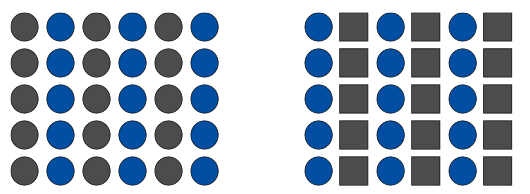
\includegraphics[scale=0.8]{img/gesetz_der_Aehnlichkeit.PNG}
  \caption{Ähnliche Objekte werden zusammengefasst.}
    \caption*{\textbf{Quelle:} \cite[59]{Dahm2006}}
  \label{fig:aehnlichkeit}
\end{figure}
Für die Ähnlichkeit sind die Farbe, die Helligkeit, die Form, das Muster und noch weitere Kriterien von Bedeutung\footnote{\cite[vgl.][59f]{Dahm2006}}. Je mehr Kriterien Elemente gemeinsam haben, desto höher ist dessen Ähnlichkeit und desto eher werden Elemente als Gruppe gesehen\footnote{\cite[vgl.][]{HTMLSeminarDe}}.

\textbf{Gesetz der Nähe}

Das Gesetz der Nähe beschreibt die Zusammengehörigkeit von Elementen durch ihre Nähe zueinander.
\begin{figure}[H]
  \centering
  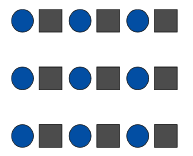
\includegraphics[scale=0.9]{img/gesetz_der_Naehe.PNG}
  \caption{Abstände zwischen Objekten erzeugen eine Zusammengehörigkeit.}
    \caption*{\textbf{Quelle:}\cite[60]{Dahm2006}}
  \label{fig:naehe}
\end{figure}
In der Abbildung \ref{fig:naehe} ist zu erkennen, dass die Elemente trotz unterschiedlicher Formen und Farben  nicht als Spalten, sondern als Zeilen, wahrgenommen werden. Dieser Effekt resultiert aus dem dominanten Merkmal der Nähe von Objekten. Die Nähe erzielt bei der Anordnung von Elementen einen noch stärkeren Effekt als die Ähnlichkeit\footnote{\cite[vgl.][60]{Dahm2006}}.


\textbf{Gesetz der Vertrautheit}

Das Gesetz der Vertrautheit beschreibt ein Phänomen, bei dem der Betrachter vertraute bzw. bekannte Formen immer wieder erkennt. Dafür sieht er aber nicht mehr die Bestandteile aus denen die Form entstanden ist.\footnote{\cite[vgl.][63f]{Dahm2006}}
\begin{figure}[H]
  \centering
  
\includegraphics[scale=0.62]{img/gesetz_der_Vertrautheit.PNG}
  \caption{Vertraute Formen bleiben beim Betrachter erhalten.}
  \caption*{\textbf{Quelle:}\cite[63]{Dahm2006}}
  \label{fig:vertrautheit}
\end{figure}
In Abbildung \ref{fig:vertrautheit} sieht der Betrachter auf den ersten Blick viele wahllos verstreute schwarze Flecken auf einem weißen Hintergrund. Wird nun die Erfahrung des Betrachters mit Informationen zu diesem Bild angereichert, wird er zukünftig diese Erfahrungen automatisch immer wieder abrufen. Dabei wird es unmöglich sein, diese Erfahrungen bewusst zu unterdrücken. In der Abbildung ist in der rechten Bildhälfte ein herabschauender Dalmatiner zu sehen. Von vielen Personen wird der Dalmatiner durch bloßes hinschauen nicht wahrgenommen. Sobald der Betrachter einmal den Dalmatiner entdeckt hat, wird er nie wieder nur wahllose Flecken sehen können.\footnote{\cite[vgl.][63f]{Dahm2006}}

%%%%%%%%%%%%%%%%%%%%%%%%%%%%%%%%%%%%%%%%%%%%%%%%%%%%%%%%%%%%%%%%%%%%%%%%%%%%

\subsubsection{Normen und Richtlinien}
\label{sec:normenUndRichtlinien}
Zu der Gestaltung und Anordnung von Elementen, gibt es eine Vielzahl von Normen und Richtlinien, die sich aus verschiedensten Arbeitsgruppen, Institutionen und Gremien entwickelt haben. Ein Grund für ihre Existenz sind die zunehmende Bedeutung von Benutzerschnittstellen und deren Gebrauchstauglichkeit und gleichzeitig auch die steigende Komplexität von Benutzerschnittstellen. Die Normen, also Anweisungen einer höheren Instanz, für das Verhalten bei gewissen Tätigkeiten, Situationen, o.Ä.\footnote{\cite[vgl.][]{duden}}, dienen als Unterstützung für die Entwicklung von einheitlichen und benutzerfreundlichen Benutzerschnittstellen. 

\textbf{Normen}

Einer dieser Software-Ergonomie Normen ist die \gls{EN} \gls{ISO} 9241. Diese wurde in ihrer ersten Auflage 1996 durch das \gls{DIN} veröffentlicht. Seitdem sind die Anforderungen und technischen Möglichkeiten immer weiter gewachsen. In dem Zuge wurde die Norm 2008 in einer überarbeiteten Fassung herausgegeben. Dabei wurden konkretere Beispiele und Empfehlungen vervielfältigt, der Nutzungskontext, der zuvor nur mit dem Blick auf PC's gerichtet war, erweitert und zusätzlich andere Normen mit einbezogen.\footnote{\cite[vgl.][]{Schneider2008}}

Der Begriff Gebrauchstauglichkeit wird in der Norm 9241-110 mit den drei Merkmalen Effektivität, Effizienz und Zufriedenheit aus der Norm 9241-11 definiert. Zudem wird im Kapitel 6 des Normteils 110 (ehemals Teil 10) die Verbindung der sieben Gestaltungsgrundsätze für ergonomische Benutzerschnittstellen (s. Tabelle \ref{tab:siebenGrundprinzipien}), aus EN ISO 9241-110 und EN ISO 9241-12, zu der Gebrauchstauglichkeit aus EN ISO 9241-11 hergestellt. Denn durch die Anwendung der sieben Grundsätze soll die Gebrauchstauglichkeit unterstützt werden.\footnote{\cite[vgl.][Kap. 6]{ISO9241-110}}

Wie in der Tabelle \ref{tab:siebenGrundprinzipien} zu erkennen ist, wurden die einzelnen Grundprinzipien in ihren Beschreibungen möglichst generisch formuliert. Ein Grund dafür ist, dass die Grundsätze unabhängig vom betrachtenden Softwaresystem angewandt werden sollen. Die Grundsätze können bei der Konzeption, Analyse und Bewertung von Dialogen angewandt werden, sollen aber keine Vorgaben an die Entwicklung von interaktiven Systemen stellen.\footnote{\cite[vgl.][Kap. 4.1]{ISO9241-110}}
\begin{center}
\begin{longtable}{|p{5.1cm}|p{9.56cm}|} 
\hline
\textbf{Grundprinzip} & \textbf{Beschreibung} \\ \hline
Aufgabenangemessenheit & Ein interaktives System ist aufgabenangemessen, wenn es den Benutzer unterstützt, seine Arbeitsaufgabe zu erledigen, d.h., wenn Funktionalität und Dialog auf den charakteristischen Eigenschaften der Arbeitsaufgabe basieren, anstatt auf der zur Aufgabenerledigung eingesetzten Technologie. \\ \hline
Selbstbeschreibungsfähigkeit & Der Dialog ist in dem Maße selbstbeschreibungsfähig, in dem für den Benutzer zu jeder Zeit offensichtlich ist, in welchem Dialog, an welcher Stelle im Dialog er sich befindet, welche Handlungen unternommen werden können und wie diese ausgeführt werden können. \\ \hline
Erwartungskonformität & Ein Dialog ist erwartungskonform, wenn er den aus dem Nutzungskontext heraus vorhersehbaren Benutzerbelangen sowie allgemein anerkannten Konventionen entspricht. \\ \hline
Lernförderlichkeit & Ein Dialog ist lernförderlich, wenn er den Benutzer beim Erlernen der Nutzung des interaktiven Systems unterstützt und anleitet. \\ \hline
Steuerbarkeit & Ein Dialog ist steuerbar, wenn der Benutzer in der Lage ist, den Dialogablauf zu starten sowie seine Richtung und Geschwindigkeit zu beeinflussen bis das Ziel erreicht ist. \\ \hline
Fehlertoleranz & Ein Dialog ist fehlertolerant, wenn das beabsichtigte Arbeitsergebnis trotz erkennbar fehlerhafter Eingaben entweder mit keinem oder mit minimalem Korrekturaufwand seitens des Benutzers erreicht werden kann. Fehlertoleranz wird mit den Mitteln erreicht: 
\begin{itemize}
  \setlength{\itemsep}{0pt}
  \setlength{\parskip}{3pt}
  \setlength{\parsep}{2pt}
  \item Fehlererkennung und -vermeidung (Schadensbegrenzung)
  \item Fehlerkorrektur oder
  \item Fehlermanagement, um mit Fehlern umzugehen, die sich ereignen.
\end{itemize} \\ \hline
Individualisierbarkeit & Ein Dialog ist individualisierbar, wenn Benutzer die Mensch-System-Interaktion und die Darstellung von Informationen ändern können, um diese an ihre individuellen Fähigkeiten und Bedürfnisse anzupassen.\\ \hline
\caption{Die sieben Grundprinzipien der Dialoggestaltung in Anlehnung an die ISO 9241-110.}
\label{tab:siebenGrundprinzipien}
\end{longtable}
\end{center}
Bei der konkreten Umsetzung sollten zunächst Merkmale der zukünftigen Benutzer, Arbeitsaufgaben, Arbeitsumgebung aber auch die zur Verfügung stehenden Technologien analysiert werden, um herauszufinden welche dieser Prinzipien im vorliegenden Kontext geeignet sind.\footnote{\cite[vgl.][]{Figl2010}}

Im Abschnitt 12 der ISO Norm 9241 werden die charakteristischen Eigenschaften der Informationsdarstellung, d.h. Klarheit, Unterscheidbarkeit, Kompaktheit, Konsistenz, Erkennbarkeit, Lesbarkeit und Verständlichkeit als unterstützendes Bindeglied für die sieben Grundsätze aus Teil 110 definiert. Insbesondere die Selbstbeschreibungsfähigkeit und Erwartungskonformität einer Benutzerschnittstelle können durch die Eigenschaften der ISO 9241-12 positiv beeinflusst werden. Insgesamt sind die Teile 110, 11 und 12 der ISO Norm 9241 eng miteinander verkettet und können positive aber auch negative Effekte aufeinander ausüben\footnote{\cite[vgl.][Kap. 6]{ISO9241-110}}. Die Wirkungsrichtungen der einzelnen Teile werden in Abbildung \ref{fig:beziehungIsoNormen} noch einmal genauer verdeutlicht.
\begin{figure}[H]
  \centering
  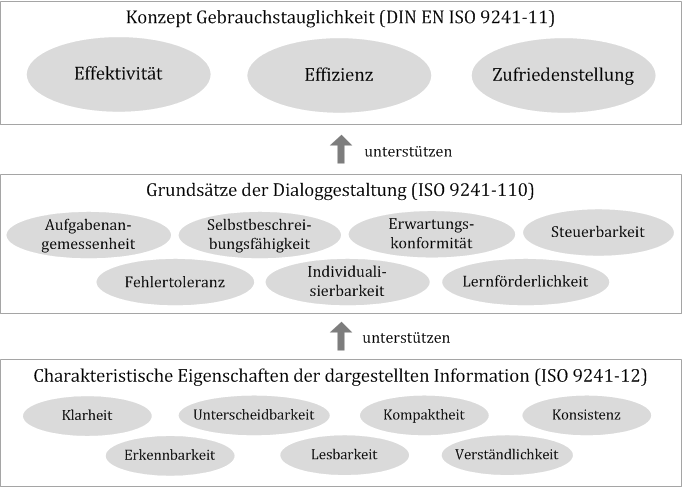
\includegraphics[scale=0.80]{img/Beziehung_ISO9241_ISO9241-11_ISO9241-12.png}
  \caption{Beziehung zwischen ISO 9241, ISO 9241-11 und ISO 9241-12.}
  \caption*{\textbf{Quelle:} Eigene Darstellung \citep[vgl.][]{ISO9241-110}}
  \label{fig:beziehungIsoNormen}
\end{figure}
Eine weitere Norm im Bereich der Software-Ergonomie, auf die im Abschnitt 3.6 in der ISO 9241-110 Norm verwiesen wird, ist die DIN EN ISO 13407 (Benutzerorientierte Gestaltung interaktiver Systeme). Diese Norm ist als Ergänzung des Teils 110, im Bereich des Projektmanagements und der Vorgehensweisen, anzusehen\footnote{\cite[vgl.][58]{Schneider2008}}.

\textbf{Richtlinien}

Zu den Richtlinien, die man bei der Software-Ergonomie berücksichtigen sollte, gehören auch die Styleguides eines Unternehmens. Dabei wird zwischen internen und externen Richtlinien unterschieden\footnote{\cite[vgl.][74]{Richter2013}}. Das Ziel dieser Styleguides ist es Systeme zu vereinheitlichen, indem gewisse Rahmenbedingungen festgelegt werden\footnote{\cite[vgl.][]{Sarodnick2011}}. Sie enthalten Vorgaben zum Aussehen und Verhalten von Bedienelementen, im jeweiligen Kontext\footnote{\cite[vgl.][72]{Richter2013}}. Jedes Unternehmen sollte gewisse Standards verfolgen, damit eine einheitliche und konsistente Weiterentwicklung und Benutzung der Software gewährleistet ist.

Der Vorteil von Styleguides liegt darin, dass dem Entwickler gewisse Denkprozesse bei der Auseinandersetzung mit Oberflächen durch die Styleguides abgenommen werden. Ebenso dienen sie auch gleichzeitig als eine Art Checkliste für den Entwickler\footnote{\cite[vgl.][214]{Thomaschewski2013}}.

Auf der anderen Seite bringen Styleguides auch per se Probleme mit sich. Beispielsweise deckt die beiliegende Dokumentation nicht alle Funktionen und Ziele ab oder es braucht mehrere Styleguides, die aber untereinander nicht konsistent sind oder die Styleguides sind nicht auf dem aktuellsten Stand. Diese Probleme erzeugen wiederum Schwierigkeiten und Probleme bei der Umsetzung\footnote{\cite[vgl.][215]{Thomaschewski2013}}. Daher sollte darauf geachtet werden, dass die Dokumentationen zu jedem Zeitpunkt aktuell und widerspruchsfrei vorzufinden sind.

%%%%%%%%%%%%%%%%%%%%%%%%%%%%%%%%%%%%%%%%%%%%%%%%%%%%%%%%%%%%%%%%%%%%%%%%%%%%

\subsubsection{Gesetze und Verordnungen}
\label{sec:gesetzeUndVerordnungen}
Neben den Gestaltgesetzen, Normen und Richtlinien, die mit ihren Empfehlungen im Designprozess unterstützen, gibt es Gesetze und Verordnungen die gewisse Vorgaben und Standards fordern. Diese sind darauf bedacht die Arbeitnehmer zu schützen und eine nationale wie auch internationale Vereinheitlichung von IT-Systemen zu fördern. Die \gls{ArbStaettV}, die anstelle der vorherigen Arbeitsschutzverordnung am 3. Dezember 2016 in Kraft getreten ist, ist einer dieser schützenden Gesetze. Die \gls{ArbStaettV} hat als Ziel Beschäftigte in Arbeitsstätten vor Arbeitsunfällen und Berufskrankheiten zu schützen. Das Gesetz enthält Mindestvorgaben an die Arbeitsstätten, die zur Sicherheit und zum Gesundheitsschutz der Beschäftigten eingeführt wurden.\footnote{\cite[vgl.][]{BAuA}}

Ein Zusammenhang des Gesetztes mit dem Thema Ergonomie wird deutlich, wenn man sich den Anlagen Teil 6 des Gesetztes anschaut. Dort lassen sich Maßnahmen und Vorgaben zur Gestaltung von Bildschirmarbeitsplätzen finden. Diese Anforderungen, wie zum Beispiel die angemessene Skalierung von Texten und Grafiken oder auch der ausreichende Kontrast von Texten und Grafiken zum Hintergrund, tragen ebenfalls zu den ergonomischen Gesichtspunkten einer gebrauchstauglichen Benutzerschnittstelle bei.\footnote{\cite[vgl.][Anhang: Kap. 6]{ArbStaettV}}

%%%%%%%%%%%%%%%%%%%%%%%%%%%%%%%%%%%%%%%%%%%%%%%%%%%%%%%%%%%%%%%%%%%%%%%%%%%%

\subsubsection{Heuristiken der Gebrauchstauglichkeit}
\label{sec:heuristikenDerGebrauchstauglichkeit}
Auf dem Gebiet der Usability von Benutzerschnittstellen und der Interaktion mit Schnittstellen, sind die Informatik Professoren Ben Shneidermann und Don Norman und der Usability Berater Dr. Jakob Nielsen, eine renommierte Referenz\footnote{\cite[vgl.][]{Wong2018}}. Ihre Vielzahl an Werken werden gerne als Referenz genutzt und ihre Erkenntnisse im Gebiet der Software-Ergonomie sind durchaus anerkannt. Diese praktikablen Ansätze und Vorgehensweisen für die Evaluation von ergonomischen Benutzerschnittstellen werden Usability Heuristiken genannt. Heuristiken sind Methoden, die auf überlieferten Verhaltensweisen und Erfahrungen basieren und dabei helfen komplexe Probleme zu lösen\footnote{\cite[vgl.][]{Heuristik2018}}. Im folgenden werden 10 Usability Heuristiken von Dr. Jakob Nielsen genannt.
\begin{itemize}
    \setlength{\itemsep}{0pt}
    \setlength{\parskip}{5pt}
    \setlength{\parsep}{3pt}
    \item Das System sollte dem Anwender immer wieder den aktuellen Status mitteilen.\footnote{\cite[vgl.][]{Nielsen1995}}
    \item Die Sprache und Ausdrucksweise des Systems sollte zu dem des Anwenders passen. Dazu zählt auch, dass Informationen in realen und logischen Reihenfolgen dargestellt werden.\footnote{\cite[vgl.][]{Nielsen1995}}
    \item Der Anwender sollte die Möglichkeit haben Aktionen zu widerrufen und erneut auszuführen. Bei kritischen Aktionen sollte erst nach einer Bestätigung der Status eines Dialoges gewechselt werden.\footnote{\cite[vgl.][]{Nielsen1995}}
    \item Die Konventionen für Syntax und Semantik sollten systemweit einheitlich eingehalten werden.\footnote{\cite[vgl.][]{Nielsen1995}}
    \item Das System sollte so konzipiert sein, dass es keine Fehlermeldungen zulässt.\footnote{\cite[vgl.][]{Nielsen1995}}
    \item Wichtige Informationen sollten jederzeit im System einsehbar sein. Hilfen zur Handhabung des Systems sollten leicht zugänglich sein.\footnote{\cite[vgl.][]{Nielsen1995}}
    \item Das System sollte sowohl für erfahrene Anwender als auch für unerfahrene Benutzer konzipiert sein.\footnote{\cite[vgl.][]{Nielsen1995}}
    \item Die Dialoge in einem System sollten immer nur wichtige Informationen anzeigen.\footnote{\cite[vgl.][]{Nielsen1995}}
    \item Fehlermeldungen sollten immer in verständlichen Inhalten für den Anwender dargestellt werden und mögliche Lösungswege vorschlagen.\footnote{\cite[vgl.][]{Nielsen1995}}
    \item Das System sollte eine ausreichende System- und Anwenderdokumentation besitzen. Außerdem sollten Informationen einfach in den Dokumentationen zu finden sein.\footnote{\cite[vgl.][]{Nielsen1995}}
\end{itemize}

Um eine all umfassendere Sicht auf mögliche Strategien und Ziele bei der Entwicklung, Analyse und Konzeption von ergonomischen Benutzerschnittstellen zu bekommen, bieten die Ansätze von Dr. Jakob Nielsen eine gute Ergänzung bzw. Erweiterung der Thematik. Eine weitere Auswahl an Usability Heuristiken stellte Ben Shneidermann mit seinen \enquote{8 Golden Rules of Interface Design}\footnote{\cite{Wong2018}} auf. Einige der dort genannten Aspekte decken sich mit den Inhalten der 10 Heuristiken von Dr. Jakob Nielsen.

%%%%%%%%%%%%%%%%%%%%%%%%%%%%%%%%%%%%%%%%%%%%%%%%%%%%%%%%%%%%%%%%%%%%%%%%%%%%

\subsubsection{Nutzen von Software-Ergonomie}
Oftmals ist Unternehmen die Wichtigkeit der Software-Ergonomie zwar bewusst, jedoch schrecken sie zurück, wenn zusätzliche Aufwände im Entwicklungsprozess aufgebracht werden müssen. Diese Kosten und Aufwände erscheinen, verglichen zum erzielten Mehrwert, oftmals für den ersten Moment zu hoch. Langfristig gesehen wird sich jedoch die Software-Ergonomie positiv auf die Produktivität auswirken. Sobald es darum geht Arbeitsabläufe zu optimieren und Zeit zu sparen sind ergonomische Softwaresysteme unabdinglich. Bezogen auf den vorliegenden Anwendungsfall bedeutet dies, dass die Produktivität und Effizienz der Sachbearbeiter unter anderem von dem Eingabedialog, mit dem zwangsweise gearbeitet werden muss, abhängt. Durch eine verbesserte Benutzerfreundlichkeit bzw. Ergonomie der \gls{GUI}, können Produktivität und Effizienz positiv beeinflusst werden. Schon wenige Sekunden Ersparnis im Arbeitsablauf eines einzelnen Sachbearbeiters, bringen einen großen Mehrwert insgesamt.\footnote{\cite[vgl.][19]{Pruemper_Harten2007}}

Die Produktivität setzt auch voraus, dass die Mitarbeiter keinen zu großen Belastungen (physisch und psychisch) ausgesetzt sind. Das heißt sowohl repetitive\footnote{repetitiv = sich wiederholend} Bewegungen der Finger, Hände, Arme und Schultern als auch der Arbeitsablauf und die Arbeitsorganisation sollten möglichst gering bzw. einfach gehalten werden. Zu hohe psychische Belastungen können daraus resultieren, dass zum Beispiel Zeitdruck, ein hoher Konzentrationsaufwand oder zu viele Unterbrechungen in den Arbeitsabläufen auftritt. Diese negativen Effekte gilt es durch eine ergonomische Software möglichst effektiv abzufangen und vorzubeugen.\footnote{\cite[vgl.][19]{Pruemper_Harten2007}}

Auch mit dem Blick auf die laufenden Kosten einer Software können langfristig große Einsparungen erreicht werden. Umso eher sich im Entwicklungsprozess mit dem Thema Software-Ergonomie auseinander gesetzt wird, desto weniger Kosten fallen später für die Erstellung der Dokumentation, die Vorbereitung und Durchführung von Schulungen und die Wartung der Software an.\footnote{\cite[vgl.][19]{Pruemper_Harten2007}}

%%%%%%%%%%%%%%%%%%%%%%%%%%%%%%%%%%%%%%%%%%%%%%%%%%%%%%%%%%%%%%%%%%%%%%%%%%%%

\subsection{Evaluation von Software-Ergonomie}
Die Evaluation im allgemeinen beschäftigt sich mit dem Sammeln und Kombinieren von Daten. Diese Daten dienen zur systematischen Auswertung und Interpretation des Evaluationsgegenstandes (z.B. Programm, Projekt, Produkt, u.a.). Für nachvollziehbare Ergebnisse, ist die Validität und Reliabilität der erhobenen Daten und Vorgehensweisen wichtig.\footnote{\cite[vgl.][7]{Hegner2003}}

%%%%%%%%%%%%%%%%%%%%%%%%%%%%%%%%%%%%%%%%%%%%%%%%%%%%%%%%%%%%%%%%%%%%%%%%%%%%

\subsubsection{Evaluationsziele}

Bei der Evaluation von Software-Ergonomie lassen sich verschiedene Ziele verfolgen. Zum Beispiel kann ein Unternehmen Interesse daran haben Software miteinander zu vergleichen, um herauszufinden welche Software besser auf sie zugeschnitten ist\footnote{\cite[vgl.][]{Gediga2002evaluation}}. In dem Fall wäre die Fragestellung \enquote{Which is better?} die Ausgangslage für die vergleichende Evaluation\footnote{\cite[vgl.][9]{Hegner2003}}. Die bewertende Evaluation ist eine weitere Herangehensweise und stellt die Frage \enquote{How good?}\footnote{\cite[vgl.][9]{Hegner2003}}. Ziel ist es eine Software hinsichtlich gewisser Kriterien und Normen zu bewerten\footnote{\cite[vgl.][]{Gediga2002evaluation}}. Die dritte Möglichkeit ist die analysierende Evaluation also \enquote{Why bad?}\footnote{\cite[vgl.][9]{Hegner2003}}, bei der das Ziel ist, die Schwachstellen eines Systems aufzudecken und Verbesserungsvorschläge aufzustellen\footnote{\cite[vgl.][]{Gediga2002evaluation}}.

%%%%%%%%%%%%%%%%%%%%%%%%%%%%%%%%%%%%%%%%%%%%%%%%%%%%%%%%%%%%%%%%%%%%%%%%%%%%

\subsubsection{Arten der Evaluation}
Bei der Art der Evaluation lässt sich zwischen der formativen Evaluation und der summativen Evaluation unterscheiden.

\textbf{Formative Evaluation}

Bei der formativen Evaluation wird mit entsprechenden Methoden möglichst früh versucht im Entwicklungsprozess anzusetzen, um eine hohe Software Qualität und damit auch Ergonomie zu erzielen. Frühzeitige Benutzerbeteiligung und Prototyping helfen dabei die Bedürfnisse der Anwender in der Software abbilden zu können. Die formative Evaluation erhebt sowohl quantitative als auch qualitative Daten. Dabei werden die quantitativen dazu genutzt die Zielerfüllung zu überprüfen. Die qualitativen Daten hingegen werden zur Ableitung von Schwächen und Verbesserungsvorschlägen verwendet. Sie kommen überwiegend in der formativen Evaluation zum Einsatz.\footnote{\cite[vgl.][7]{Hegner2003}}

\textbf{Summative Evaluation}

Die summative Evaluation ist darauf ausgerichtet Software miteinander zu vergleichen oder Hypothesen und Erwartungen zu überprüfen. Dazu könnte eine Software zum Beispiel an gewissen Kriterien gemessen werden, die zu Anfang aufgestellt wurden. Die Verfahren zur Erhebung von empirischen Daten stammen überwiegend aus dem quantitativen Bereich, wie zum Beispiel die Befragungsmethode des Fragebogens (siehe Kap. \ref{sec:erhebungsmethoden}).\footnote{\cite[vgl.][8]{Hegner2003}}

%%%%%%%%%%%%%%%%%%%%%%%%%%%%%%%%%%%%%%%%%%%%%%%%%%%%%%%%%%%%%%%%%%%%%%%%%%%%

\subsubsection{Erhebungsmethoden}
\label{sec:erhebungsmethoden}
Bei der Evaluation im Bereich der Software gibt es verschiedene Methodiken und Vorgehensweisen, mit denen sich Daten erheben lassen. Diese erhobenen Daten sind im Evaluationsprozess von Bedeutung. Je nach Ziel, Benutzergruppe, Ort, Art der Informationen und Ressourcen, fällt die Wahl einer Evaluationsmethode unterschiedlich aus\footnote{\cite[vgl.][10]{Hegner2003}} und somit auch die Art der Erhebung. Die Ausrichtung einer Erhebungsmethode lässt sich von objektiv über empirisch und analytisch bis hin zu subjektiv einordnen\footnote{\cite[vgl.][15]{Hegner2003}}.

\textbf{Objektive Methoden}

Bei den objektiven Methoden ist es das Ziel, \enquote{harte} Daten zu erheben und zu bewerten. Diese harten Daten werden durch die bloße Beobachtung des Evaluationsgegenstandes ermittelt. Die Daten liegen in strukturierter Form vor und sind unabhängig von der subjektiven Wahrnehmung der Benutzer. Die objektiven Methoden zielen auf Daten, wie zum Beispiel die Bearbeitungszeit oder Fehlerraten, ab und eigenen sich eher zum Vergleich von zwei Systemen. Jedoch besitzen diese Methoden keinerlei Kontextinformationen und sind somit nicht für die Erarbeitung von Verbesserungsvorschlägen geeignet.\footnote{\cite[vgl.][17]{Hegner2003}}

\textbf{Subjektive Methoden}

Subjektive Methoden versuchen möglichst nah bei den Eindrücken und Erfahrungen der Benutzern anzusetzen. Dabei werden Meinungen und Einschätzungen der Benutzer eingeholt, um den zu evaluierenden Gegenstand zu bewerten. Die erhobenen Daten zählen zu den \enquote{weichen} Daten. Die subjektiven Methoden sind in ihrer Durchführung mit eher geringem Aufwand verbunden, jedoch kann die nachfolgende Auswertung, bei umfangreichen Antworten, sehr zeitintensiv sein.\footnote{\cite[vgl.][18]{Hegner2003}}

Man kann sagen, dass beide Arten von Methoden ihre Vor- und Nachteile besitzen, daher ist es oftmals sinnvoll die Methodiken miteinander zu kombinieren. Dadurch werden Schwächen mancher Methoden durch Stärken anderer ausgeglichen\footnote{\cite[vgl.][261]{Pruemper1997}}. In der Abbildung \ref{fig:erhebungsmethodenObjektivitaetBenutzerbeteiligung} wird noch einmal verdeutlicht, welche Erhebungsmethoden existieren und wie diese im Kontext der Objektivität bzw. Subjektivität und der dazu stehenden Benutzerbeteiligung einzuordnen sind.
\begin{figure}[H]
  \centering
  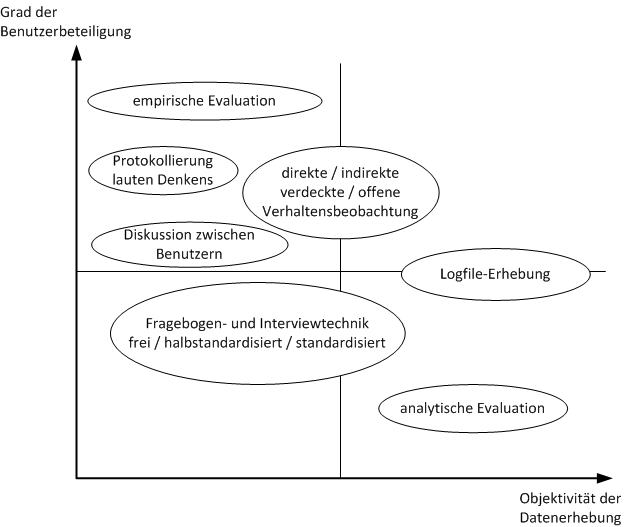
\includegraphics[scale=0.8]{img/Datenerhebungsmethoden_Objektivitaet_Benutzerbeteiligung.png}
  \caption{Vergleich von Erhebungsmethoden aufgrund des Grades der Benutzerbeteiligung und der Objektivität der Methode.}
  \caption*{\textbf{Quelle:} Eigene Darstellung \citep[vgl.][16]{Hegner2003}}
  \label{fig:erhebungsmethodenObjektivitaetBenutzerbeteiligung}
\end{figure}
Man kann sehen, dass sich die Methoden teilweise nicht genau einer Kategorie zuordnen lassen. Daher wurden zwischen der Subjektivität und der Objektivität noch die Formen der analytischen (leitfadenorientierten) und der empirischen Evaluation eingeführt\footnote{\cite[vgl.][15]{Hegner2003}}.

Im folgenden werden explizit nur die Erhebungsmethoden vorgestellt und eingeordnet, die im Zuge dieser Ausarbeitung zum Einsatz kamen.

\textbf{Logfile-Erhebung}

Eine Methode zur Erhebung objektiver Daten ist die Logfile-Erhebung. Bei der Methode werden die Daten automatisch durch ein Erfassungssystem erhoben. Interaktionen, die Benutzer mit dem System erzeugen, werden vollständig aufgezeichnet. Beispielsweise werden Zeiten zwischen Interaktionen oder die Häufigkeit von Maus- und Tastaturanschlägen gemessen\footnote{\cite[vgl.][63]{Hegner2003}}. Diese Methode der Erhebung bietet eine effiziente und kostengünstige Aufzeichnung von Beobachtungsdaten\footnote{\cite[vgl.][Kap. 65.3]{Baur2014}}. Da die Logfile-Erhebung keine Kontextinformationen erfasst und rein objektive Daten wie z.B. Maus- oder Tastaturanschläge aufzeichnet, bietet sich eine Kombination mit einer Befragungsmethode wie z.B. dem Fragebogen an\footnote{\cite[vgl.][17\psq]{Hegner2003}}.

\textbf{Fragebogen}

Eine subjektive jedoch in Teilen auch objektive Methode ist der standardisierte Fragebogen. Hierbei werden von den Benutzern Meinungen, Erfahrungen und Einschätzungen zum untersuchenden Evaluationsgegenstand eingeholt. Das Ergebnis eines Fragebogens kann durch eine Häufigkeitsauswertung von freien und vorgegebenen Antworten ermittelt werden. Je freier eine Frage beantwortet werden darf, umso vielfältiger wird das Antwortenspektrum. Auf der anderen Seite sinkt bei steigender Freiheit die Bereitschaft der Befragten zu antworten und bestenfalls auch konstruktiv zu antworten. Im Bereich der Usability gibt es mehrere standardisierte Fragebögen wie den Questionnarie for User Interaction Satisfaction (QUIS), den IsoMetrics oder den Isonorm 9241/10 Fragebogen, welcher nachfolgend genauer vorgestellt wird.\footnote{\cite[vgl.][Kap. 4.5.1.1]{Hegner2003}}

Der aus dem deutschsprachigen Raum stammende Isonorm 9241/10 Fragebogen, wurde wie auch der IsoMetrics Fragebogen, basierend auf der EN ISO 9241-110 entwickelt. Sein Fragenkatalog unterteilt sich in sieben Kriterien, die äquivalent zu den Gestaltungsgrundsätzen der EN ISO 9241-10 sind. Mit fünf Items pro Kriterium besitzt der Fragebogen insgesamt 35 Items. Jede der Aussagen wird auf einer 7-stelligen Rating-Skala (siehe Abb. \ref{fig:IsonormBewertungsskala}) bewertet, die von sehr negativ (\enquote{$---$}) bis sehr positiv (\enquote{$+++$}) reicht\footnote{\cite[vgl.][Kap. 3.3]{Figl2010}}. 
\begin{figure}[H]
  \centering
  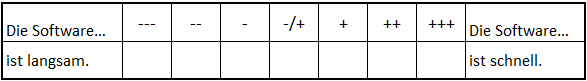
\includegraphics[scale=0.95]{img/Isonorm_Bewertungsskala.PNG}
  \caption{Bewertungsskala des Isonorm 9241/110 Fragebogens.}
  \caption*{\textbf{Quelle:} Eigene Darstellung}
  \label{fig:IsonormBewertungsskala}
\end{figure}
Mit einer etwa 10 minütigen Bearbeitungszeit, eignet sich der Isonorm Fragebogen besonders bei der Frage: \enquote{Entspricht die Software den Kriterien der EN ISO 9241-110 Norm?}. Zudem lässt er sich gut in iterative Softwareprozesse einbringen, indem er für eine schnelle Evaluierung der einzelnen Prototypen eingesetzt wird\footnote{\cite[vgl.][Kap. 3.3]{Figl2010}}.

\textbf{Interview}

Zu den qualitativen Erhebungsmethoden in der empirischen Sozialforschung zählen die Interviews. Diese können aufgrund ihres Grades an Strukturiertheit, der Art des Kontaktaufnahme, der Gruppengröße und dem Autoritätsanspruch des Interviewers in unterschiedlichen Formen vorliegen\footnote{\cite[vgl.][61]{Hegner2003}}. Die Spannweite dabei reicht von sehr offenen Interviews, bei denen weder die Fragen noch die Reihenfolge festgelegt sind, bis hin zu sehr strukturierten Interviews wie dem \enquote{Teacher Relationship Interview}, bei dem Fragen, Nachfragen und deren Reihenfolge vorgegeben werden. Allgemein sind Interviews dann interessant, wenn neue Erkenntnisse oder Meinungen zu einem Thema eingeholt werden sollen. Der Vorteil dabei ist, dass die Befragten Freiräume bekommen, um ihre Meinungen, Sichtweisen und Orientierungen zu äußern\footnote{\cite[vgl.][52\psqq]{Kelle2008}}. Auf der anderen Seite führen Interviews bedeutend höhere Kostenaufwände mit sich, als beispielsweise schriftliche Befragungen\footnote{\cite[vgl.][62\psq]{Hegner2003}}.

%%%%%%%%%%%%%%%%%%%%%%%%%%%%%%%%%%%%%%%%%%%%%%%%%%%%%%%%%%%%%%%%%%%%%%%%%%%%

\subsubsection{Gütekriterien für Erhebungsmethoden}

Die Güte oder auch Qualität einer Erhebungsmethode wird anhand der drei Hauptgütekriterien Objektivität, Validität und Reliabilität bewertet. Darüber hinaus gibt es auch noch weitere Nebengütekriterien (z.B. Normierung, Ökonomie oder Nützlichkeit)\footnote{\cite[vgl.][Kap. 3.5]{Figl2010}} auf die im Folgenden jedoch nicht genauer eingegangen werden wird.

Die Objektivität sagt aus, ob ein Testergebnis unabhängig von der Testperson ist. Bedeutet, dass verschiedene Personen, die gleichen Testergebnisse erzielen\footnote{\cite[vgl.][Kap. 1]{Himme2007}}. Dieses Kriterium wird, im Fall des Isonorm Fragebogens, durch die standardisiert vorgegebenen Antwortmöglichkeiten und die Auswertungsvorschriften für die Ergebnisse gewährleistet\footnote{\cite[vgl.][Kap. 3.5.1]{Figl2010}}.

Die Validität gibt an, inwiefern ein Messinstrument gültig ist bzw. die benötigte Genauigkeit besitzt. Es wird überprüft, ob das Gemessene, dem entspricht, was gemessen werden soll\footnote{\cite[vgl][Kap. 1]{Himme2007}}. Dabei lässt sich bei der Validität zwischen Inhalts-, Kriteriums und Konstruktvalidität unterscheiden. In allen drei Bereichen zeigt der Isonorm Fragebogen eine ausreichende Erfüllung der Anforderungen\footnote{\cite[vgl.][Kap. 3.5.2]{Figl2010}}.

Als drittes Qualitätsmerkmal wird die Reliabilität herangezogen. Diese beschreibt die Zuverlässigkeit und Stabilität eines Messinstruments. Um eine hohe Zuverlässigkeit bei der Erhebung von Daten zu erreichen, müssen unter anderem gemessene Ergebnisse durch erneutes Messen reproduzierbar sein\footnote{\cite[vgl.][Kap. 1]{Himme2007}}. Der Isonorm Fragebogen weist sowohl eine gute innere Konsistenz als auch eine hohe Retest-Reliabilität auf\footnote{\cite[vgl.][Kap. 3.5.3]{Figl2010}}. Die Logfile-Erhebung weist, durch eine hohe Automatisierung, generell eine höhere Reliabilität als ein Fragebogen auf\footnote{\cite[vgl.][Kap. 65.3]{Baur2014}}.

%%%%%%%%%%%%%%%%%%%%%%%%%%%%%%%%%%%%%%%%%%%%%%%%%%%%%%%%%%%%%%%%%%%%%%%%%%%%

\subsubsection{Grundbegriffe der Statistik}
\textbf{Grundgesamtheit und Stichprobe}

Immer wenn es in der Statistik um die Analyse von Daten geht, bei denen die Menge von Bedeutung sind, fallen in diesem Zusammenhang Begriffe wie Grundgesamtheit oder Stichprobe. Die Grundgesamtheit hängt von der betrachteten Einheit ab, über die statistische Aussagen getroffen werden sollen und beschreibt die mögliche Menge dieser Einheit\footnote{\cite[vgl.][13]{Statistik2016}}.

Da die Einbeziehung der Gesamtheit typischerweise nicht möglich ist, wird die Erhebung bzw. Analyse auf gewisse Kriterien und somit auf einen Teil der Grundgesamtheit eingeschränkt. In dem Fall wird von einer Teilgesamtheit oder Stichprobe gesprochen\footnote{\cite[vgl.][13]{Statistik2016}}.

\textbf{Statistische Einheit, Merkmal und Merkmalsausprägung}

Wird erneut das Beispiel mit der Schule und den Schülern betrachtet, dann ist die statistische Einheit in diesem Kontext ein einzelner Schüler. Sollte zum Beispiel die Anzahl der Fenster in der Schule ermitteln werden, dann ist die zu untersuchende statistische Einheit beziehungsweise der Merkmalsträger das Fenster.\footnote{\cite[vgl.][13]{Statistik2016}}

Die Eigenschaften einer Einheit wird Merkmal genannt. Mögliche Merkmale, die bei einer Analyse von Schülern untersucht werden können sind Körpergröße, Augenfarbe, Haarfarbe oder Geschlecht. Merkmale können verschiedene Merkmalsausprägungen annehmen. Es kann zwischen qualitativen und quantitativen Ausprägungen unterschieden werden. Beispielsweise ist die Körpergröße ein Merkmal mit quantitativen Ausprägungen, in dem Fall sind alle natürlichen Zahlen größer null möglich. Eine qualitatives Merkmal hingegen ist beispielsweise das Geschlecht, das nur zwei Ausprägungen annehmen kann entweder Mann oder Frau.\footnote{\cite[vgl.][13\psqq]{Statistik2016}}

Grundlegend wird bei Merkmalen und ihren Ausprägungen zwischen drei verschiedenen Skalen zum Messen der Merkmale und ihren Ausprägungen unterschieden. Die Nominalskala stellt das niedrigste Skalenniveau der drei Skalen dar und wird zur Klassifizierung und Darstellung von qualitativen Merkmalsausprägungen verwendet. Merkmale, die dieser Skala angehören, können lediglich gezählt und in der Häufigkeit ihrer Ausprägungen dargestellt werden.\footnote{\cite[vgl.][15\psqq]{Statistik2016}}

Das nächst höhere Skalenniveau wird durch die Ordinalskala abgebildet. Beispielsweise gehören Schulnoten (Ausprägungen: sehr gut, gut, befriedigend, ausreichend, mangelhaft und ungenügend) zur Ordinalskala, die neben den Anwendungsgebieten der Nominalskala auch zum Vergleichen von Ausprägungen genutzt werden kann.\footnote{\cite[vgl.][15\psqq]{Statistik2016}}

Die Intervallskala besitzt nicht nur das höchste Skalenniveau, sondern ist auch am vielfältigsten bei der Berechnung von Lageparametern. Diese werden im nächsten Abschnitt genauer erläutert. Die Intervallskala kann neben dem Vergleichen von Merkmalsausprägungen, auch einen numerischen Unterschied zwischen zwei Ausprägungen ermitteln.\footnote{\cite[vgl.][15\psqq]{Statistik2016}}

%%%%%%%%%%%%%%%%%%%%%%%%%%%%%%%%%%%%%%%%%%%%%%%%%%%%%%%%%%%%%%%%%%%%%%%%%%%%

\subsection{Usability-Engineering}
\subsubsection{Vorgehensmodell}
\label{sec:vorgehensmodellUsabilityEngineering}
Usability-Engineering ist ein Vorgehen, das mit Hilfe eines Vorgehensmodell und dazugehörigen Methoden, bei der Entwicklung von benutzerfreundlicher Software unterstützt. Dabei ist ein Vorgehensmodell eine definierte Abfolge von Prozessschritten, die während des Entwicklungsprozesses durchlaufen werden\footnote{\cite[vgl.][7]{Richter2013}}. Generell lässt sich bei Vorgehensmodellen in der Entwicklung zwischen konventionellen und agilen Modellen unterscheiden. Zu den konventionellen oder auch klassischen Ansätzen zählen zum Beispiel das Wasserfallmodell\footnote{\cite[vgl.][27\psqq]{Brandt2008}}. Die klassischen Modelle sind meist einfach zu verstehen aber durch ihre sequenzielle\ Abfolge von Prozessschritten eher unflexibel in der Handhabung.

Agile Vorgehensmodelle, wie zum Beispiel das Spiralmodell oder \gls{XP}, folgen einem iterativen Ansatz. Im Entwicklungsprozess bedeutet das, dass mehrmals gleiche Phasen bzw. Tätigkeiten durchlaufen werden können und keine vordefinierte Reihenfolge eingehalten werden muss\footnote{\cite[vgl.][29\psqq]{Brandt2008}}. Grundsätzlich werden beim Usability-Engineering das Umfeld (Nutzungskontext), die Arbeitsabläufe, geeignete Funktionalitäten und Konzepte zu den grafischen Benutzeroberflächen analysiert und erarbeitet. Dabei hat sich das Usability-Engineering zum Ziel gemacht, komplexe Strukturen zu vereinfachen und eine Lösung zu entwerfen, die genau auf die Anforderungen der Benutzergruppe angepasst ist\footnote{\cite[vgl.][7]{Richter2013}}. Somit bietet sich das Vorgehen gut bei der Entwicklung von grafischen Benutzeroberflächen an, da die Benutzer mit ihren Rückmeldungen ein fester Bestandteil der Entwicklungsphase sind.

Die EN ISO 9241-210 hat das Usability-Engineering als Standardvorgehen bei der Entwicklung von ergonomischer Software etabliert. Das Modell besitzt einen hohen Abstraktionsgrad und lässt sich daher für verschiedene Projekttypen einsetzen\footnote{\cite[vgl.][21]{Ecker2016}}. In der Abbildung \ref{fig:usabilityEngineeringVorgehensmodell} werden die vier Hauptphasen des Usability-Engineerings nach ISO 9241-210 dargestellt und nachfolgend erläutert.
\begin{figure}[H]
  \centering
  \fbox{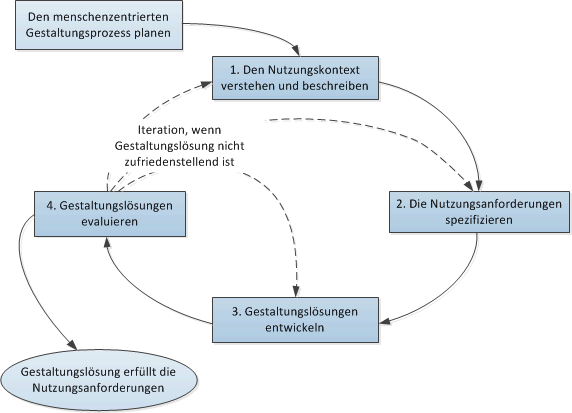
\includegraphics[scale=1]{img/Usability_Engineering_Vorgehensmodell.png}}
  \caption{Usability-Engineering Prozessmodell in Anlehnung an DIN EN ISO 9241-210.}
  \caption*{\textbf{Quelle:} Eigene Darstellung}
  \label{fig:usabilityEngineeringVorgehensmodell}
\end{figure}
\begin{enumerate}
    \item In der ersten Phase des Software Projektes geht es darum, den Nutzungskontext (siehe Kap. 4.4.2) möglichst voll umfassend zu verstehen und zu beschreiben. Zum Nutzungskontext gehören die betroffenen Benutzergruppen mit deren Tätigkeiten und Arbeitsabläufen und die Arbeitsumgebung selbst. Die benötigten Informationen lassen sich mit Hilfe von Erhebungsmethoden (siehe Kap. 4.3.3) wie z.B. Fragebögen oder persönlichen Interviews eruieren\footnote{\cite[vgl.][28\psq]{Ecker2016}}.
    \item In der zweiten Phase des Modells werden die Anforderungen der betroffenen Benutzergruppen analysiert und dokumentiert. Dazu gehört, dass sich der Projektleiter mit den Benutzern und deren Sichtweise auseinander setzt und die Anforderungen zusammen erarbeitet werden\footnote{\cite[vgl.][30\psq]{Ecker2016}}.
    \item Im dritten Prozessschritt werden die definierten Anforderungen in Form von Prototypen oder Mock-ups\footnote{Ein Mock-up ist eine oftmals zu präsentationszwecken grafisch modellierte Attrappe eines Produkts.} ausgearbeitet. In der Phase werden Entwürfe sowohl von der Ablaufsteuerung als auch vom Oberflächendesign erstellt. Die Ablaufsteuerung beinhaltet die wechselseitige Interaktion zwischen Benutzer und Software. Diese Abläufe werden in geeignete Schnittstellen oder Prozessdiagramme abgebildet. Der zweite Teil der Entwicklung besteht aus dem Entwurf der \gls{GUI}. Dazu gehört, dass die Interaktionsart (Maus, Tastatur, etc.) mit der Schnittstelle festgelegt wird und dementsprechend geeignete Bedienelemente ausgewählt und ergonomisch angeordnet werden\footnote{\cite[vgl.][33\psq]{Ecker2016}}.
    \item Im vierten Schritt werden die Gestaltungslösungen aus dem vorherigen Schritt evaluiert. Die Benutzer bewerten die entworfenen Mock-ups, Skizzen oder die fertig implementierte Schnittstelle, um Mängel oder Fehler frühzeitig zu erkennen. Für die Bewertung der Gestaltungslösungen sind Benutzungstests, Fragebögen oder Fokusgruppen\footnote{Eine Art der Gruppendiskussion, bei der moderierte und leitfadenorientierte Fragen diskutiert werden.} mögliche Herangehensweisen. Sollte keiner der Gestaltungslösungen die Nutzungsanforderungen ausreichend erfüllen, so können iterativ vorherige Phasen durchlaufen werden\footnote{\cite[vgl.][34\psq]{Ecker2016}}. Hingegen kann der Entwicklungsprozess bei befriedigender Lösung beendet und die finale Gestaltungslösung ausgerollt werden.
\end{enumerate}

\subsubsection{Analysemethoden}
\label{sec:analysemethoden}
Während des Entwicklungsprozesses gibt es mehrere Techniken mit denen die Gestaltungslösungen analysiert und evaluiert werden können. Unter anderem lassen sich auch die in Kapitel \ref{sec:erhebungsmethoden} vorgestellten Methoden der Befragung mittels Fragebogen oder das Interview anwenden. 

Als weitere Möglichkeit gibt es die Einbeziehung von Experten. Dazu zählt die Methode der heuristischen Evaluation, bei der Gestaltungslösungen anhand aufgestellter Empfehlungen, Normen und Gesetze (siehe Kap. \ref{sec:gestaltgesetze}, \ref{sec:normenUndRichtlinien}, \ref{sec:gesetzeUndVerordnungen} und \ref{sec:heuristikenDerGebrauchstauglichkeit}) bewertet werden. Diese Methode vernachlässigt jedoch die Benutzerbedürfnisse und eignet sich daher eher als ergänzende Methode.\footnote{\cite[vgl.][249]{Nielsen1990}}

Eine weitere benutzerbezogene Methode ist \enquote{Thinking Aloud}. Bei dieser Methode werden wenige Benutzer mit Video und Ton aufgenommen und sollen ihre Gedanken und Probleme während der Bearbeitung von gezielten Aufgabenstellungen äußern. Dadurch sollen Schwachstellen und Probleme beim Umgang mit dem System hervorgehen.\footnote{\cite[vgl.][51]{Hegner2003}}

%%%%%%%%%%%%%%%%%%%%%%%%%%%%%%%%%%%%%%%%%%%%%%%%%%%%%%%%%%%%%%%%%%%%%%%%%%%%

\subsubsection{Nutzungskontext}
Der Nutzungskontext muss im Zuge der zweiten Phase aus dem Vorgehensmodell nach ISO 9241-210 analysiert werden. Der Nutzungskontext setzt sich aus den betroffenen Benutzergruppen, den umliegenden Arbeitsabläufen und dem technischen Umfeld zusammen. Diese Bestandteile sollen im Folgenden genauer erläutert werden.

\textbf{Benutzergruppen}

Einen Teil der Kontextanalyse beinhaltet die Erhebung von Merkmalen der Benutzer. Zu den Merkmalen, die durchaus einen Einfluss auf die Entwicklung des interaktiven Systems nehmen können, gehören Kenntnisse, Fertigkeiten, Erfahrungen, Ausbildung, Übungsgrad, physische Merkmale sowie motorische und sensorische Fähigkeiten\footnote{\cite[vgl.][28]{Ecker2016}}. Die unterschiedlichen Ausprägungen der Benutzer (insofern diese gegeben sind) sollten ebenso mit in den Entwicklungsprozess einfließen.

\textbf{Arbeitsabläufe}

Ebenso spielen für den Entwurf der Benutzerschnittstelle die Ausprägungen der Arbeitsabläufe eine Rolle. Typischerweise sollte neben dem Erfassen der Tätigkeiten und ihrem Zusammenspiel auch die Dauer und Häufigkeit betrachtet werden\footnote{\cite[vgl.][28]{Ecker2016}}.

\textbf{Technisches Umfeld}

Zu Erhebung des technischen Umfelds, lässt sich generell zwischen der Software und der Hardware unterscheiden. Die Software manifestiert sich zum Beispiel im Betriebssystem der Benutzer, dass durchaus Unterschiede aufweisen kann. Hingegen werden zur Hardware jegliche Hilfsmittel am Arbeitsplatz wie Monitore, Drucker oder Taschenrechner gezählt und aufgenommen.\footnote{\cite[vgl.][28]{Ecker2016}}

%%%%%%%%%%%%%%%%%%%%%%%%%%%%%%%%%%%%%%%%%%%%%%%%%%%%%%%%%%%%%%%%%%%%%%%%%%%%
